\documentclass[11pt]{article}


% --- Packages ---
\usepackage{amsmath, amsthm, amsfonts, amssymb, hyperref, soul, latexsym, stmaryrd, booktabs} % fonts and characters
\usepackage{enumitem, ytableau, comment, graphicx, makecell, appendix, titling, scrextend, float, multirow, placeins, subcaption} % utilities
\usepackage{tikz, tikz-cd, tikzsymbols, pgfplots} % plots crap
\pgfplotsset{compat=1.18}
\usepackage{blkarray} % random math 
\usepackage{pstricks,pst-node,pst-tree} % networks
\usepackage{verbatim} % write code
\newlength\myverbindent % indent code
\setlength\myverbindent{0.5in} % change this to change indentation
\makeatletter
\def\verbatim@processline{%
  \hspace{\myverbindent}\the\verbatim@line\par}


% --- Matplotlib ---
% we import figures as pgfplots, which means its exported as tex to matplotlib
% to do this, we need certain commands in the premable to compile the way it shoud
\def\mathdefault#1{#1}
\everymath=\expandafter{\the\everymath\displaystyle}
\makeatletter\@ifpackageloaded{underscore}{}{\usepackage[strings]{underscore}}\makeatother


% --- Formatting ---
\usepackage{fullpage} % margins
\usepackage{setspace}
\doublespacing

\numberwithin{equation}{section} % number equations with section number
\numberwithin{figure}{section} % number figure with section number
\numberwithin{table}{section} % number table with section number


% --- Math Crap ---
\newcommand{\E}{\mathbb{E}}
\newcommand{\Z}{\mathbb{Z}}
\newcommand{\R}{\mathbb{R}}
\newcommand{\Q}{\mathbb{Q}}
\newcommand{\C}{\mathbb{C}}
\newcommand{\N}{\mathbb{N}}
\newcommand{\lagr}{\mathcal{L}}
\newcommand{\e}{\varepsilon}
\renewcommand{\sup}{\text{sup}}
\renewcommand{\inf}{\text{inf}}
\renewcommand{\d}{\delta}
\renewcommand{\Re}{\text{Re}}
\renewcommand{\Im}{\text{Im}}
\newcommand{\Arg}{\text{Arg}}
\newcommand{\Var}{\mathrm{Var}}
\newcommand{\Cov}{\mathrm{Cov}}


% --- Bibliography ---
\usepackage[style=apa, backend=biber, ibidtracker=false]{biblatex} % packages
\bibliography{sources} % .bib file


% --- Title ---
\title{Estimating Fiscal Multipliers: An SVAR Approach}
\author{Gavin Engelstad\thanks{Replication code available at \url{https://github.com/GavinEngelstad/SVAR-Fiscal-Multiplier}.} \\ \href{mailto:gengelst@macalester.edu}{gengelst@macalester.edu} \and Samina Stack \\ \href{mailto:sstack@macalester.edu}{sstack@macalester.edu}}
\date{Fall 2024}

%% --- Document ---
\begin{document}

\maketitle

\begin{abstract}
    TBD
\end{abstract}

%% --- Paper Sections ---
% --- Introduction ---
\section{Introduction} \label{sec:intro}
 %importance of good fiscal policy

 %Regulation of economy is important (political economy stuff??)
Monetary and fiscal policy are the two main channels through which the US economy is regulated.  Monetary policy involves the central bank exercising power over the aggregate money supply to change interest rates in an effort to impact consumption decisions.  Fiscal policy describes the federal government's efforts to affect the economy through the two main mechanisms of public spending and taxes.  
% Competing effects necessitate an optimal policy mix 

%Need some transition to just talking about fiscal

%how the multiplier factors into this

Competing theories of the effect of fiscal policy on output exist.  While the general IS-LM model predicts an increase in government spending to have an expansionary effect on output, standard real business cycle (RBC) models predict the opposite depending on assumptions of non-Ricardian versus Ricardian consumers \parencite{gali2007understanding}.  It is important that policymakers understand the effects of a given policy as, for example, prolonged budget deficits can have significant negative effects on long-run economic outcomes through reduced national savings and higher interest rates \parencite{gale2003economic}.

We estimate the effect of government spending on the economy with the fiscal multiplier, which measures the change in output in response to a change in fiscal policy \parencite{spilimbergo2009fiscal}.  The theory of the Keynesian multiplier suggests the multiplier is greater than one, meaning every dollar change in fiscal policy causes more than a dollar change in output through households and businesses spending the additional money provided by the government \parencite{barro2011macroeconomic}.  Alternatively, the theory of crowding out suggests rational-acting households respond to increases in spending by saving more since they know fiscal forces will need to readjust later, suggesting a multiplier less than one \parencite{berge2021fiscal}.  Estimates of the multiplier inform policymakers on the effect of their decisions, so an accurate understanding of how the multiplier effects work is important \parencite{eyraud2013challenge}.  Biased estimates of the multiplier have used to guide policy during financial crises have hampered economic recovery \parencites{blanchard2013growth}{blanchard2014learning}.  A higher multiplier suggests very different optimal policy decisions than a lower one, especially in times of economic crisis.  In this paper, we estimate a multiplier around one using historical data on the US economy, suggesting increases in government spending cause an almost equal increase in output.

Economists use a variety of tools to estimate the multiplier. Quantitative modeling approaches, which use mathematical equations calibrated to match real decision-making processes to model the behavior of economic agents, tend to estimate a multiplier between 0.5 and 1 \parencite{gechert2012fiscal}. Standard statistical approaches use regressions, instrumental variables, and likelihood estimation find a multiplier between 0.25 and 0.75 \parencite{gechert2012fiscal}. This paper uses a structural vector autoregression (VAR) to estimate the multiplier effect.

Originating from \textcite{sims1980macroeconomics}, structural VARs introduce structural restrictions to reduced-form VAR models which allow for a causal interpretation of the estimates.  This general framework has been applied to study postwar business cycle fluctuations, oil shocks, and the effect of monetary policy regime on output \parencites{hamilton1983oil}{hodrick1997postwar}{sims2006were}. Our paper is based on the framework in \textcite{blanchard2002empirical}, which presents a structural VAR approach to estimate the fiscal multiplier. 


% --- Lit Review ---
\section{Lit Review} \label{sec:lit}

Previous studies suggest underestimation of the multiplier led to misestimation of growth during financial crises \parencite{blanchard2013growth}.  

Increasing taxes reduces GDP \parencite{barro2011macroeconomic}

Understanding multiplier helps us understand short-term effects of fiscal policy \parencite{eyraud2013challenge}.

Stage of business cycle changes size of multiplier \parencite{baum2012fiscal}.


Structural parameters for Uhlig's restrictions fail to satisfy restrictions on systematic components of monetary policy \parencite{arias2019systematic}.

Implications on income inequality when incorporating expectations.  Unanticipated fiscal consolidations can lead to long-term increases in inequality \parencite{furceri2022distributional}

As steady state debt level increases, so too does the debt multiplier \parencite{albonico2021public}.  (Implications for fiscal policy during recessions)

Spending multiplier larger during periods of low economic activity while tax multipliers larger during periods of high economic activity \parencite{arin2015fiscal}


Multiplier estimated through
\begin{itemize}
    \item using one through seven quarter ahead forecasts of key macroeconomic variables such as consumption, output, and wages to control for agents' information sets \parencite{hall2023economic}
\end{itemize}


Estimate of multiplier depends heavily on method of estimation \parencite{gechert2012fiscal}.




% --- Empirical Strategy ---
\section{Empirical Strategy} \label{sec:emp}
\subsection{Growth Versus Business Cycle Effects} \label{subsec:detrend}

Economists separate movements of the into two distinct categories: growth effects and business cycle effects \parencite{stulz1985macroeconomic}. Growth effects, typically measured using decade to decade long-run economic trends, are determined by a country's pace of idea generation, strength of institutions, and other more stagnant factors \parencites{acemoglu2001colonial}{jones2016facts}{jones2019paul}. Business cycles, in contrast, include short-run economic fluctuations caused by policy decisions, international events, and other unpredictable shocks \parencites{lucas1995understanding}{mitchell2024business}. This paper exclusively focuses on understanding the business cycle consequences of fiscal policy.

\begin{figure}[t]
    \centering
    \caption{US real GDP per capita over time (1952-2007)}
    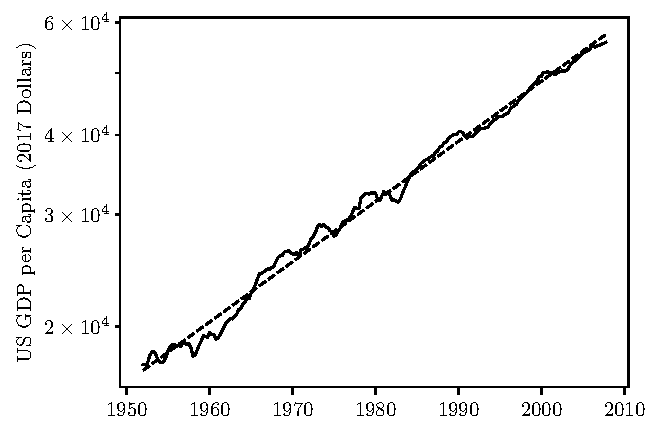
\includegraphics{figures/growth_effects.pdf}

    {\scriptsize \emph{Notes:} Dashed best fit line calculated using OLS.}
    \label{fig:growth-effects}
\end{figure}

Figure \ref{fig:growth-effects} shows US real GDP per capita from 1952 to 2007. Over time, long-run growth is very consistent and follows a linear-in-logs trend. This long-run constant growth is well-documented across the world in growth rates for key macroeconomic indicators \parencites{papell2014long}.\footnote{There have been a handful of instances where this breaks, including the so-called ``growth miracles'' in East Asia \parencite{easterly199511} and the post-Great Recession growth slowdowns \parencites{benigno2018stagnation}. For the purposes of this paper, we treat long-run constant growth as a fact.} This constant trend is also key for isolating business cycle effects; fluctuations around the constant growth path can be viewed as exclusively business cycle effects.

Numerically, for an economic indicator $y_t$ we use the log-deviation from trend $\hat{y}_t$ as its business cycle effect. To calculate this, we run the regression
\[
    \log y_t = \alpha_0 + \alpha_1 t + \hat{y}_t
\]
where $\alpha_0$ and $\alpha_1$ determine the long-run trend for the indicator and the error term $\hat{y}_t$ is the indicator's business cycle deviations from the trend \parencite{seip2024scoring}.\footnote{For interpretability, we multiply this by 100 in all of our results and figures. Since deviations from trend, at least within the United States, are small, this can be thought of as the ``percent deviation from trend'' of the indicator.} This method can be overly simplistic for data the exhibits significant changes in growth rates over time, but our exclusive focus on the effect of policy decisions within the United States, a country that has exhibited consistent trends over time, avoids these concerns.


\subsection{The Reduced-Form VAR}

\begin{figure}[t!]
    \centering
    \caption{Order one, three variable, reduced-form VAR causal graph}
    \begin{psmatrix}[colsep=1.5cm, rowsep=1cm]
    % nodes
    $\dots$ & $y_{1, t-3}$ & $y_{1, t-2}$ & $y_{1, t-1}$ & $y_{1, t}$ \\
    $\dots$ & $y_{2, t-3}$ & $y_{2, t-2}$ & $y_{2, t-1}$ & $y_{2, t}$ \\
    $\dots$ & $y_{3, t-3}$ & $y_{3, t-2}$ & $y_{3, t-1}$ & $y_{3, t}$

    % first column of arrows
    \ncline[nodesep=5pt]{->}{1,1}{1,2}
    \ncline[nodesep=5pt]{->}{1,1}{2,2}
    \ncline[nodesep=5pt]{->}{1,1}{3,2}
    \ncline[nodesep=5pt]{->}{2,1}{1,2}
    \ncline[nodesep=5pt]{->}{2,1}{2,2}
    \ncline[nodesep=5pt]{->}{2,1}{3,2}
    \ncline[nodesep=5pt]{->}{3,1}{1,2}
    \ncline[nodesep=5pt]{->}{3,1}{2,2}
    \ncline[nodesep=5pt]{->}{3,1}{3,2}

    % second column
    \ncline[nodesep=5pt]{->}{1,2}{1,3}
    \ncline[nodesep=5pt]{->}{1,2}{2,3}
    \ncline[nodesep=5pt]{->}{1,2}{3,3}
    \ncline[nodesep=5pt]{->}{2,2}{1,3}
    \ncline[nodesep=5pt]{->}{2,2}{2,3}
    \ncline[nodesep=5pt]{->}{2,2}{3,3}
    \ncline[nodesep=5pt]{->}{3,2}{1,3}
    \ncline[nodesep=5pt]{->}{3,2}{2,3}
    \ncline[nodesep=5pt]{->}{3,2}{3,3}

    % third column
    \ncline[nodesep=5pt]{->}{1,3}{1,4}
    \ncline[nodesep=5pt]{->}{1,3}{2,4}
    \ncline[nodesep=5pt]{->}{1,3}{3,4}
    \ncline[nodesep=5pt]{->}{2,3}{1,4}
    \ncline[nodesep=5pt]{->}{2,3}{2,4}
    \ncline[nodesep=5pt]{->}{2,3}{3,4}
    \ncline[nodesep=5pt]{->}{3,3}{1,4}
    \ncline[nodesep=5pt]{->}{3,3}{2,4}
    \ncline[nodesep=5pt]{->}{3,3}{3,4}

    % second column
    \ncline[nodesep=5pt]{->}{1,4}{1,5}
    \ncline[nodesep=5pt]{->}{1,4}{2,5}
    \ncline[nodesep=5pt]{->}{1,4}{3,5}
    \ncline[nodesep=5pt]{->}{2,4}{1,5}
    \ncline[nodesep=5pt]{->}{2,4}{2,5}
    \ncline[nodesep=5pt]{->}{2,4}{3,5}
    \ncline[nodesep=5pt]{->}{3,4}{1,5}
    \ncline[nodesep=5pt]{->}{3,4}{2,5}
    \ncline[nodesep=5pt]{->}{3,4}{3,5}
\end{psmatrix}

    \label{fig:rfvar-graph}
\end{figure}

Our strategy to estimate the causal effect of fiscal policy decisions on GDP is based on VARs. The reduced-form of a VAR assumes a vector of outputs follows an autoregressive process with respect to the whole vector \parencite{neusser2016time}. Like standard univariate autoregressive models, the order of the VAR determines the number of lags included in the model. Unlike univariate autoregressive models, we model a variable using lags for the full set of outputs in the model, not just one.

Figure \ref{fig:rfvar-graph} demonstrates the assumed causal graph for a three variable, order one VAR. At each time $t$, the whole vector of outputs $Y_t = (y_{1, t}, y_{2, t}, y_{3, t})'$ depends on the whole vector at time $t-1$. Causal pathways lead from $y_{1, t-1}$, $y_{2, t-1}$, and $y_{3, t-1}$ into $y_{t,1}$. A higher order VAR would extend this so $Y_t$ depends on more past versions of itself. For example, a second order model would assume $Y_t$ depends on $Y_{t-1}$ and $Y_{t-2}$.

The estimating equation for an order $p$ VAR with $n$ outputs is given by
\[
    Y_t = \sum_{\ell = 1}^p B_\ell Y_{t - \ell} + u_t
\]
where $Y_t$ is the $n \times 1$ vector of outputs we are interested in modeling, $B_{t - \ell}$ is the $n \times n$ coefficient matrix, and $u_t$ is the $n \times 1$ vector of multivariate-normal error terms with variance-covariance matrix $\Sigma$. The terms in $u_t$ represent exogenous shocks to the variables in the model, including international events and movements in excluded macroeconomic indicators.


\subsection{Correlated and Structural Shocks}

Reduced form VARs are effective tools for understanding associations between variables and for forecasting, but fail to differentiate between causation and correlation \parencite{stock2001vector}. This is because the covariance terms in the variance-covariance matrix $\Sigma$ are symmetric. Therefore, the error term includes the effects of both contemporaneous relationships between the variables in the model when one is shocked and structural shocks, or exogenous shocks to the outputs in the model. Therefore, reduced form VARs only have a causal interpretation when variables are assumed to have no contemporaneous causal relationships.

In macroeconomics, fluctuations in macroeconomic series are assumed to be very interrelated \parencites{sims1980macroeconomics}{shapiro1988sources}{blanchard1988dynamic}{cochrane1994shocks}{nakamura2018identification}. The FED sets the interest rate based on the opinions and forecasts of hundreds of economists about the current state of the economy, so understanding how the interest rate affects the economy requires separating the contemporaneous effect of the state of the economy on the interest rate from the effect of the interest rate on the economy \parencite{nakamura2018identification}. Variation in the interest rate standard statistical methods would identify off of could be caused by changes in the overall economy, obscuring the actual effect.

To determine the causal effect of fiscal policy on output, we will need to separate these contemporaneous relationships from actual structural shocks. Forward-looking household behavior, tax schemes that take a fraction of incomes, and revenue-based spending decisions by policymakers mean many of these contemporaneous relationships exist that will confound this relationship \parencites{blanchard2002empirical}{gali2020effects}.


\subsection{Structural VAR} \label{subsec:svar}

To isolate the effects of structural shocks from contemporaneous relationships, we use a structural VAR. A structural VAR adds an additional coefficient matrix to the left-hand side of the estimating equation to get
\[
    A_0 Y_t = \sum_{\ell = 1}^p A_\ell Y_{t - \ell} + \varepsilon_t
\]
where $A_0$ is the matrix of contemporaneous relationships, $A_\ell = A_0 B_\ell$ is the matrix of lagged coefficients, and $\varepsilon_t = A_0 u_t$ is the structural error term \parencite{neusser2016time}. Unlike the reduced-form error term, the variance-covariance matrix of the structural error term is the $n \times n$ identity matrix $I_n$.\footnote{Normalizing the variances to 1 is not strictly necessary; identification only requires the covariances to be zero. The benefit to this normalization is that when we shock the model we measure the effects of a ``typical'' shock.}

To fit the structural VAR, we need to assume which relationships exist within the contemporaneous matrix $A_0$. Specifically, we need to fix $\begin{pmatrix} n \\ 2 \end{pmatrix}$ coefficients within this matrix and can estimate the remaining coefficients as simultaneous relationships \parencite{neusser2016time}. Importantly, within certain $A_0$ matrix structures, a series can be contemporaneously affected by a structural shock to a series we do not enforce a relationship with through some intermediate factor. These feedback effects within the matrix are the benefit to SVAR estimation, which calculates $A_0$ using the $\Sigma$ matrix, as opposed to row-wise OLS estimation.

\begin{figure}[t!]
    \centering
    \caption{Order one, three variable, structural VAR causal graph}
    \begin{psmatrix}[colsep=1.5cm, rowsep=1cm]
    % nodes
    $\dots$ & $y_{1, t-3}$ & $y_{1, t-2}$ & $y_{1, t-1}$ & $y_{1, t}$ \\
    $\dots$ & $y_{2, t-3}$ & $y_{2, t-2}$ & $y_{2, t-1}$ & $y_{2, t}$ \\
    $\dots$ & $y_{3, t-3}$ & $y_{3, t-2}$ & $y_{3, t-1}$ & $y_{3, t}$

    % first column of arrows
    \ncline[nodesep=5pt]{->}{1,1}{1,2}
    \ncline[nodesep=5pt]{->}{1,1}{2,2}
    \ncline[nodesep=5pt]{->}{1,1}{3,2}
    \ncline[nodesep=5pt]{->}{2,1}{1,2}
    \ncline[nodesep=5pt]{->}{2,1}{2,2}
    \ncline[nodesep=5pt]{->}{2,1}{3,2}
    \ncline[nodesep=5pt]{->}{3,1}{1,2}
    \ncline[nodesep=5pt]{->}{3,1}{2,2}
    \ncline[nodesep=5pt]{->}{3,1}{3,2}
    \ncline[nodesep=5pt]{->}{1,2}{2,2}
    \ncarc[nodesep=5pt,arcangle=-15]{->}{2,2}{3,2}
    \ncarc[nodesep=5pt,arcangle=-15]{->}{3,2}{2,2}

    % second column
    \ncline[nodesep=5pt]{->}{1,2}{1,3}
    \ncline[nodesep=5pt]{->}{1,2}{2,3}
    \ncline[nodesep=5pt]{->}{1,2}{3,3}
    \ncline[nodesep=5pt]{->}{2,2}{1,3}
    \ncline[nodesep=5pt]{->}{2,2}{2,3}
    \ncline[nodesep=5pt]{->}{2,2}{3,3}
    \ncline[nodesep=5pt]{->}{3,2}{1,3}
    \ncline[nodesep=5pt]{->}{3,2}{2,3}
    \ncline[nodesep=5pt]{->}{3,2}{3,3}
    \ncline[nodesep=5pt]{->}{1,3}{2,3}
    \ncarc[nodesep=5pt,arcangle=-15]{->}{2,3}{3,3}
    \ncarc[nodesep=5pt,arcangle=-15]{->}{3,3}{2,3}

    % third column
    \ncline[nodesep=5pt]{->}{1,3}{1,4}
    \ncline[nodesep=5pt]{->}{1,3}{2,4}
    \ncline[nodesep=5pt]{->}{1,3}{3,4}
    \ncline[nodesep=5pt]{->}{2,3}{1,4}
    \ncline[nodesep=5pt]{->}{2,3}{2,4}
    \ncline[nodesep=5pt]{->}{2,3}{3,4}
    \ncline[nodesep=5pt]{->}{3,3}{1,4}
    \ncline[nodesep=5pt]{->}{3,3}{2,4}
    \ncline[nodesep=5pt]{->}{3,3}{3,4}
    \ncline[nodesep=5pt]{->}{1,4}{2,4}
    \ncarc[nodesep=5pt,arcangle=-15]{->}{2,4}{3,4}
    \ncarc[nodesep=5pt,arcangle=-15]{->}{3,4}{2,4}

    % second column
    \ncline[nodesep=5pt]{->}{1,4}{1,5}
    \ncline[nodesep=5pt]{->}{1,4}{2,5}
    \ncline[nodesep=5pt]{->}{1,4}{3,5}
    \ncline[nodesep=5pt]{->}{2,4}{1,5}
    \ncline[nodesep=5pt]{->}{2,4}{2,5}
    \ncline[nodesep=5pt]{->}{2,4}{3,5}
    \ncline[nodesep=5pt]{->}{3,4}{1,5}
    \ncline[nodesep=5pt]{->}{3,4}{2,5}
    \ncline[nodesep=5pt]{->}{3,4}{3,5}
    \ncline[nodesep=5pt]{->}{1,5}{2,5}
    \ncarc[nodesep=5pt,arcangle=-15]{->}{2,5}{3,5}
    \ncarc[nodesep=5pt,arcangle=-15]{->}{3,5}{2,5}
\end{psmatrix}

    \label{fig:svar-graph}
\end{figure}

An example causal graph for a structural VAR is shown in Figure \ref{fig:svar-graph}. Since the output vector has three series, we can enforce three simultaneous relationships. In the example, we enforce that $y_1$ causes $y_2$, $y_2$ causes $y_3$, and $y_3$ causes $y_2$. Identification restrictions for the structural VAR can estimate causal effects even along cyclical causal paths. A structural shock to $y_1$ could affect $y_3$ through $y_2$ and a structural shock to $y_2$ would impact $y_2$ through both direct effects from the shock and indirect effects through $y_2$.


\subsection{Estimating Fiscal Multipliers}

To estimate the effect of a fiscal shock, we estimate the reduced form VAR
\[
    Y_t = \sum_{\ell = 1}^p B_\ell Y_{t - 1} + u_t
\]
where $Y_t = (x_t, g_t, t_t)'$ is a vector of GDP $X_t$, government spending $G_t$, and government revenue $T_t$. Since our data is quarterly, in our preferred specification we use $p = 4$ corresponding to a total period of one year. We choose this since taxes are often paid at an annual frequency, so including one year of lags captures the relevant revenue data over the entire time span \parencite{blanchard2002empirical}. The error term $u_t = (u_t^x, u_t^g, u_t^t)$ has nonzero covariance, meaning the relationships predicted by the VAR and within the coefficient matrices $B_\ell$ are correlations and not causal.

To identify the causal effect, we implement the model from \textcite{blanchard2002empirical}. We assume
\begin{align*}
    u_t^x &= a_1 u_t^g + a_2 u_t^t + \varepsilon_t^x \\
    u_t^g &= b_1 u_t^x + b_2 \varepsilon_t^t + \varepsilon_t^g \\
    u_t^t &= c_1 u_t^x + c_2 \varepsilon_t^g + \varepsilon_t^t
\end{align*}
where $\varepsilon = (\varepsilon_t^x, \varepsilon_t^g, \varepsilon_t^t)'$ is the vector of mutually uncorrelated structural shocks.\footnote{Technically, to fit this system within the framework from Section \ref{subsec:svar} it would need to be rearranged. This formulation is known as the ``AB-model,'' which allows for two structural shocks to show up in the same equation \parencite{lutkepohl2005new}. The interpretations and general concepts of the ``AB-model'' and ``A-model'' introduced earlier are identical, so we ignore this difference.} The first equation enforces unexpected movements in GDP can be caused by unexpected movements in government spending, government revenue, or structural shocks to GDP. The second enforces that unexpected movements in government spending are caused by unexpected movements in GDP or structural shocks to government revenue or spending. The third equation enforces that unexpected movements in government revenue are caused by unexpected movements in GDP or structural shocks to government spending or revenue.

As is, this system is underidentified, meaning we need to add additional conditions to make the model estimatable. We follow the procedure from \textcite{blanchard2002empirical} that has become standard when estimating the fiscal multiplier \parencites{ramey2011can}{caldara2017analytics}{deleidi2021quantifying}. First, we set $b_1 = 0$. This assumption is justified by the lack of automatic stabilizers for government spending in the US economy \parencites{caldara2017analytics}. Then, we fix $c_1$ using external estimates for the response of government revenue to economic activity. Following \textcite{lutz2010fiscal}, we set $c_1 = 1.7$. Finally, to differentiate between government spending and revenue structural shocks, we set either $b_2$ or $c_2$ to 0. Like \textcite{blanchard2002empirical}, we present two alternative specifications: one where $b_2 = 0$ meaning government spending is decided before revenue and another where $c_2 = 0$ meaning government revenue is decided before spending. Figure \ref{fig:causal-graph} shows a causal graph for the pathways between the estimated structural shocks and unexpected movements in the outcomes of interest. The causal pathways affecting GDP, government revenue, and government spending therefore include the pathways affecting unexpected movements in Figure \ref{fig:causal-graph} as well as the autoregressive precesses.

\begin{figure}[t]
    \centering
    \caption{Causal graph for unexpected movements in GDP, government spending, and revenue}
    \begin{psmatrix}[colsep=3cm, rowsep=1cm]
    % nodes
    $u_t^x$ & $\varepsilon_t^x$ \\
    $u_t^g$ & $\varepsilon_t^g$ \\
    $u_t^t$ & $\varepsilon_t^t$

    % first column of arrows
    \ncline[nodesep=5pt]{->}{2,1}{1,1}
    \ncarc[nodesep=5pt,arcangle=15]{->}{3,1}{1,1}
    \ncarc[nodesep=5pt,arcangle=-25,linewidth=1.5pt]{->}{1,1}{3,1}
    \ncline[nodesep=5pt]{->}{1,2}{1,1}
    \ncline[nodesep=5pt]{->}{2,2}{2,1}
    \ncline[nodesep=5pt]{->}{3,2}{3,1}
    \ncline[nodesep=5pt,linestyle=dashed,dash=3pt 2pt]{->}{2,2}{3,1}
    \ncline[nodesep=5pt,linestyle=dashed,dash=3pt 2pt]{->}{3,2}{2,1}
\end{psmatrix}

    \label{fig:causal-graph}
\end{figure}

This identification strategy relies on many assumptions about the structure of the causal relationships between movements and structural shocks. An alternative strategy from \textcite{mountford2009effects} instead imposes a penalty function on the long-run effects of a structural shock. Estimations using this approach tend to be similar to those using the \textcite{blanchard2002empirical} method we employ. Other strategies that impose conditions on the reduced form of the VAR using sign restrictions or Bayesian techniques but allow for identification of the structural shocks under a weaker set of assumptions are outside the scope of this paper.


% --- Data ---
\section{Data} \label{sec:data}
To estimate the effect, we use data on GDP, government spending, and government revenue from FRED between 1960Q1 and 2007Q4. The upper end of the estimations window is chosen due to changes in growth trends post-2008, though we believe with a more robust detrending procedure we would observe similar business cycle effects during the post-2008 period \parencite{benigno2018stagnation}.

\begin{figure}[t!]
    \centering
    \caption{Detrended data series for GDP, government spending, and government revenue}
    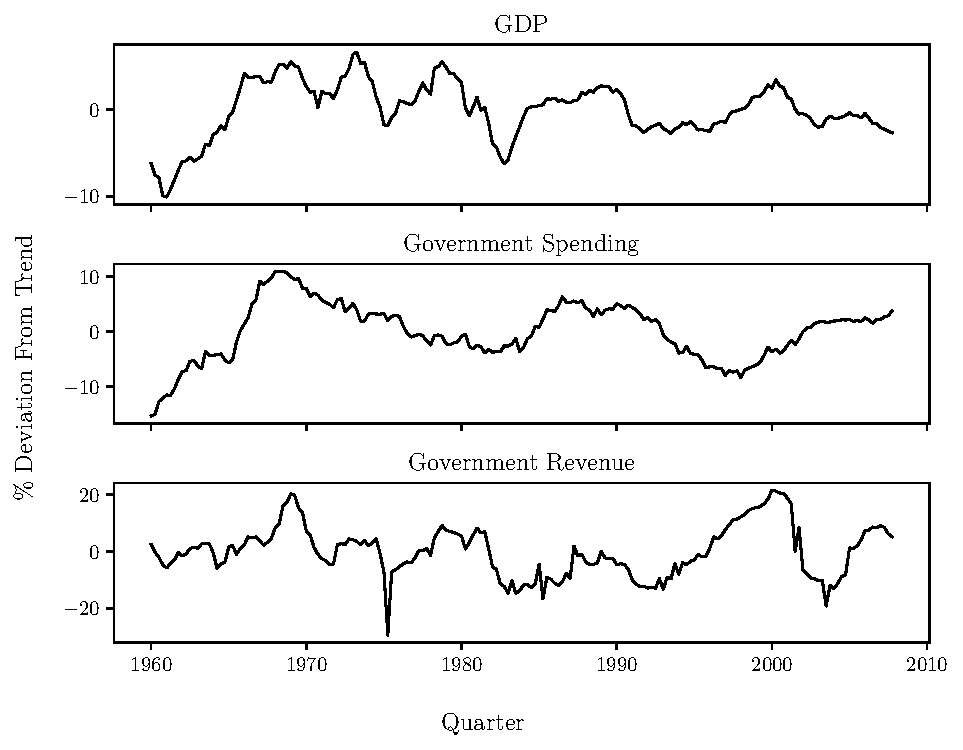
\includegraphics{figures/detrended_data.pdf}
    \label{fig:dta}
\end{figure}

We use the `Gross Domestic Product' series for GDP, `Government Consumption Expenditures and Gross Investment' series for government spending, and the `Federal Government Current Tax Receipts' series for government revenue. Each series is then divided by the GDP Deflator to convert it to real terms instead of nominal, then detrended according to the procedure in \ref{subsec:detrend}. Detrended series throughout the period are shown in Figure \ref{fig:dta}.


% --- Results ---
\section{Results} \label{sec:results}
\begin{table}[t]
    \centering
    \caption{Estimated structural parameters}
    \begin{tabular}{ccc}
    \toprule
    & (1) & (2) \\
    & $b_2 = 0$ & $c_2 = 0$ \\
    \midrule
    $a_1$ & -0.182 & -0.182 \\
    $a_2$ & -0.150 & -0.150 \\
    $b_2$ && 0.040 \\
    $c_2$ & 0.826 \\
    \bottomrule
\end{tabular}

    \label{tab:results}
\end{table}

Table \ref{tab:results} shows the estimated values for $a_1$, $a_2$, $b_2$, and $c_2$ under both specifications. The estimated coefficients for $a_1$ and $a_2$ are virtually identical across both specifications, which justifies the assumption that we can zero out one of them and still measure the actual effect. The signs and magnitudes of our estimates are comparable to those found in other literature, including \textcite{blanchard2002empirical}.

One benefit to modeling an autoregressive process is the ability to observe the causal effect of a shock at time $t$ at later time periods. Because of the detrending process, the model has a 0 steady state for all three series. Starting from this steady state, we apply a government spending structural shock to the model that increases spending by 1\%. Then, the predictions at time $t$ are used for lags at time $t + 1$. Iterating this process gets the impulse response function (IRF), which shows the behavior of the model after the shock.

\begin{figure}[t!]
    \centering
    \caption{Estimated IRFs for a structural government spending shock}
    \begin{subfigure}{\textwidth}
        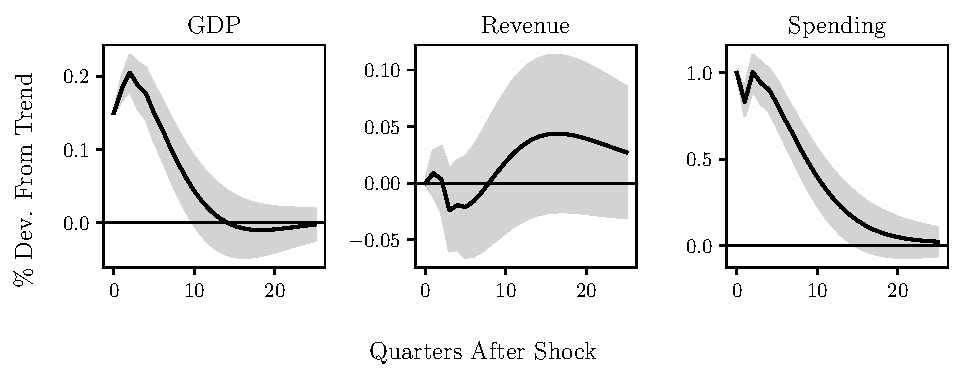
\includegraphics{figures/b20_irf.pdf}
        \caption{$b_2 = 0$}
    \end{subfigure}

    \begin{subfigure}{\textwidth}
        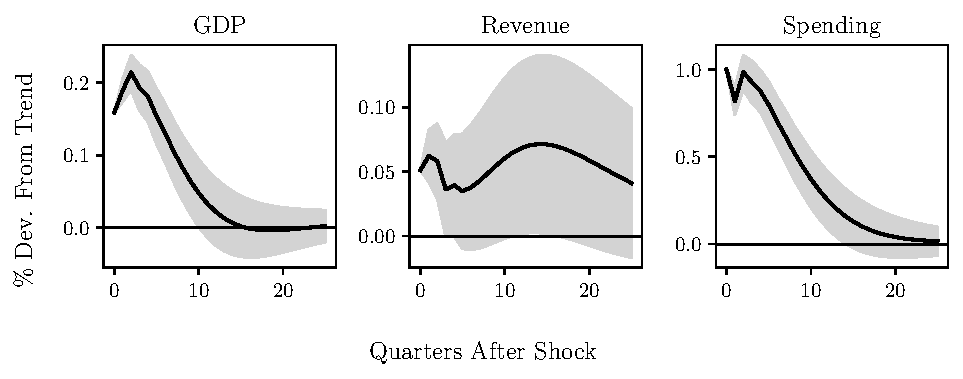
\includegraphics{figures/c20_irf.pdf}
        \caption{$c_2 = 0$}
    \end{subfigure}

    {\scriptsize \emph{Notes:} IRFs iterated for 25 periods.}
    \label{fig:irfs}
\end{figure}

Figure \ref{fig:irfs} shows the estimated IRFs for the two models. GDP and government spending follow the same paths across both specifications, again supporting the robustness of our results. Government revenues vary more between specifications but are both within the uncertainty interval of each other. The eigenvalues of the system have a magnitude less than one, so all three series eventually trend towards the steady state, demonstrating the short-run effects of business cycles \parencite{mitchell2024business}. Because government spending is shocked, it responds immediately. The largest increase in GDP happens slightly after the shock hits, meaning causal effect of the shock is delayed. The effect on government revenue happens much later, consistent with the idea that most government spending is deficit financed in the short run, then paid back well into the future \parencite{haley1941federal}.

Following \textcite{blanchard2002empirical}, the causal effect of the government spending shock is the maximum effect along the IRF. An alternative approach would examine the integral of the whole curve, but since GDP is a flow, not stock, variable, we view the single period increase as more important \parencite{deleidi2023government}. The causal effect is adjusted by the average GDP to government spending ratio to get the dollar effect on GDP of a dollar increase in government spending.

The $b_2 = 0$ model predicts a \$1 structural shock to government spending would increase GDP by \$0.990 with a standard error of \$0.115 and the $c_2 = 0$ model predicts the shock would increase GDP by \$1.035 with a standard error of \$0.115. Since GDP includes government spending, both estimates suggest the GDP effect of the spending shock is entirely the spending increase from the shock. Therefore, we find no evidence of either crowding-out or multiplier effects.


% --- Robustness ---
\section{Robustness} \label{sec:robust}
In this section, we examine four potential issues with our analysis. We test an alternative responsiveness of government revenue to economic activity, different VAR orders, and whether the multiplier changes over time. 


\subsection{Government Revenue Response}

In our main analysis, we use a government revenue responsiveness to GDP changes of 1.7 based on \textcite{lutz2010fiscal}, which is different from the 2.08 value used in \textcite{blanchard2002empirical}. The 1.7 value is based on more updated data and methods, but we want to ensure this assumption is not driving all of our results. Therefore, we estimate the model with $c_1 = 2.08$.

\begin{table}[t]
    \centering
    \caption{Estimated parameters and multiplier when $c_1 = 2.08$}
    \begin{tabular}{lcc}
    \toprule
    & (1) & (2) \\
    & $b_2 = 0$ & $c_2 = 0$ \\
    \midrule
    \emph{Parameters} \\
    \quad $a_1$ & -0.177 & -0.177 \\
    \quad $a_2$ & -0.163 & -0.163 \\
    \quad $b_2$ && 0.041 \\
    \quad $c_2$ & 0.919 \\
    \midrule
    \emph{Multiplier} \\
    \quad Estimate & 1.079 & 1.126 \\
    \quad Std. Err. & 0.115 & 0.115 \\
    \quad Time & 2 & 2 \\
    \bottomrule
\end{tabular}
    \label{tab:new-c1}
\end{table}

The results of this are in Table \ref{tab:new-c1}. The estimated parameters are almost identical to the earlier results in Table \ref{tab:results}. In both specifications, the $a_1$ and $a_2$ parameters are within 0.02 of those estimated earlier. The estimated multiplier is slightly higher, suggesting a 7-12\% multiplier effect, but still happens after a slight delay and is (almost) within a standard error of 1 where no multiplier effect exists.


\subsection{VAR Order}

The results in Section \ref{sec:results} use a fourth order VAR. We justify this choice using the taxation window that affects government revenue, but the causal effect should be robust to changes in the autoregressive order of the model. We test this by calculating the multiplier using a VAR with orders between 1 and 24, corresponding to a window between 1 quarter and 6 years.

\begin{figure}[t]
    \centering
    \caption{Estimated multiplier for different VAR orders}
    \begin{subfigure}{0.475\textwidth}
        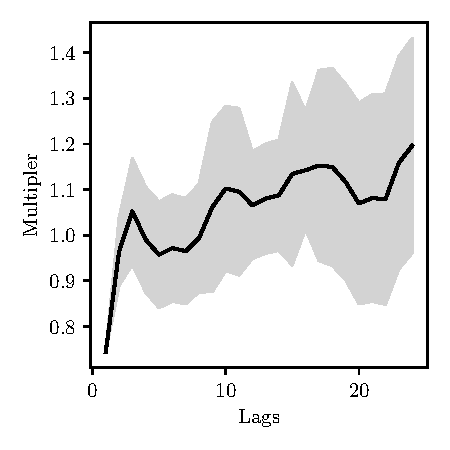
\includegraphics{figures/b20_lags.pdf}
        \caption{$b_2 = 0$}
    \end{subfigure}
    \begin{subfigure}{0.475\textwidth}
        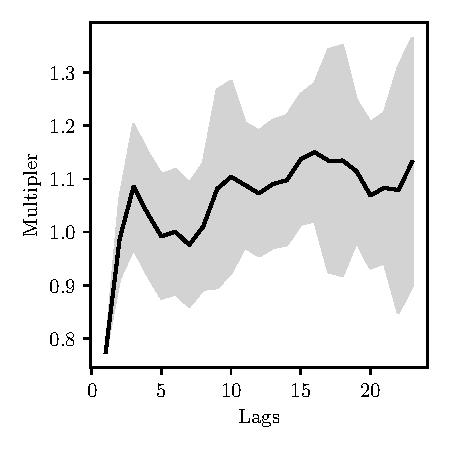
\includegraphics{figures/c20_lags.pdf}
        \caption{$c_2 = 0$}
    \end{subfigure}
    \label{fig:orders}
\end{figure}

The multiplier estimate for models with a different number of lags is shown in Figure \ref{fig:orders}. With only one lag, the estimate is much lower than our specification from Section \ref{sec:results} gets. However, the models that include more than one lag all estimate similar effects that are within the error interval of each other. Therefore, our order choice for the VAR does not determine our findings, and the causal effect is robust to different reasonable order choices.


\subsection{Temporal Trends in the Multiplier}

Our analysis in Section \ref{sec:results} assumes the multiplier is constant throughout the estimation window. We test this by estimating a separate multiplier for shorter periods within the estimation window. Specifically, we estimate the multiplier over a decade-long period at 2.5-year intervals from 1947 to 2019. This extends the estimation window on both ends, so we also test the assumption that our multiplier estimates are meaningful after the estimation window, though that does mean the estimations are less meaningful during the 50s which had significantly larger government revenue and spending volatility and during estimation windows that include 2007 and 2008 due to the different growth trends during the period.

\begin{figure}[t]
    \centering
    \caption{Estimated multiplier for different estimation windows}
    \begin{subfigure}{0.475\textwidth}
        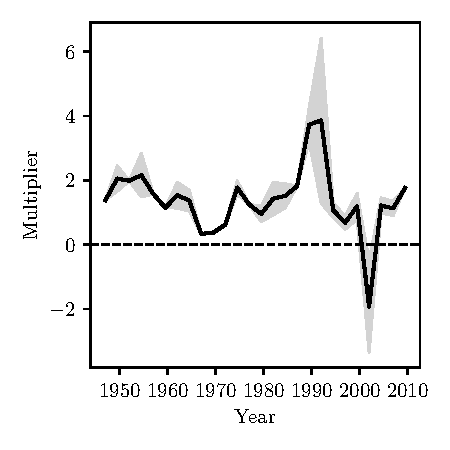
\includegraphics{figures/b20_ts.pdf}
        \caption{$b_2 = 0$}
    \end{subfigure}
    \begin{subfigure}{0.475\textwidth}
        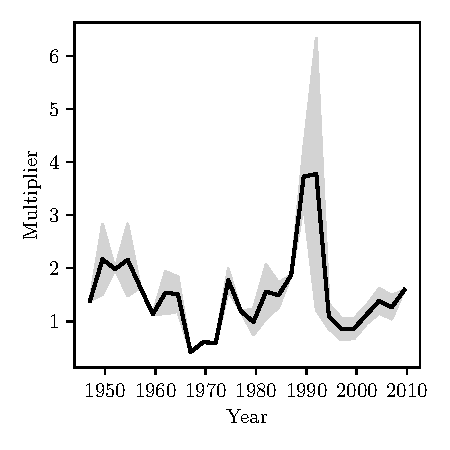
\includegraphics{figures/c20_ts.pdf}
        \caption{$c_2 = 0$}
    \end{subfigure}

    {\scriptsize \emph{Notes:} Multiplier calculated within a 10-year estimation windows that starts at the quarter on the x-axis.}
    \label{fig:ts}
\end{figure}

Figure \ref{fig:ts} shows the evolution of the multiplier over time. As expected, the estimates do not make sense in estimation windows that include 2007 and 2008 and are elevated pre-1960. Within the 1960 to 2007 estimation window, the multiplier hovers around our estimated value throughout most of the period, though does decrease in the late 60s and increase in the early 90s. Post-2008, the multiplier is near one in both specifications, suggesting our results could represent more recent business cycle forces. 

% time heterogenaity (2007+?)
% More/less lags
% Use 2.08 instead of 1.7 (follow blanchard perrotti)
% Fed funds rate?

% --- Conclusion ---
\section{Conclusion} \label{sec:concl}
This paper estimates the fiscal multiplier using a structural VAR. We impose a simultaneous relationship between GDP, government spending, and revenue à la \textcite{blanchard2002empirical}. Then, we analyze the effect of a structural government spending shock. Analysis of the GDP response to a spending shock finds a \$1 increase in government spending causes a slightly delayed approximate \$1 increase in GDP. This result is robust to minor specification changes and, ignoring specific years at the end of the 60s and start of the 90s, is relatively consistent over time.

Our analysis relies on key assumptions about the structure of macroeconomic relationships. We assume government spending has a delayed response to changes in GDP, a certain value for the government revenue response to GDP changes, and need to impose additional identification restrictions to uncover the causal effect. Our estimate is robust to minor changes in these assumptions, but we do not test our estimate against specifications that impose a completely different set of structural VAR assumptions. These could include long-run conditions that allow more simultaneous relationships to be estimated, sign restrictions, or Bayesian priors \parencites{mountford2009effects}{afonso2019fiscal}.

There is also evidence that the multiplier effect evolves over time in response to macroeconomic events. Particularly, estimates suggest the size of the multiplier changes throughout the business cycle \parencites{baum2012fiscal}{albonico2021public}. Specifically, spending multipliers are larger during periods of low economic activity \parencite{arin2015fiscal}. This would suggest the volatility seen in Figure \ref{fig:ts} is not noise, and could represent a real change in the multiplier.

Still, we believe our structural VAR approach does reasonably well at estimating the fiscal multiplier. Future work could address this paper's limitations with alternative structural frameworks. It could also analyze heterogeneity in the multiplier, either over time, across different states, or between different countries. Additionally, economic theory suggests the revenue-side multiplier, which this paper ignores, should behave similarly to the spending-side multiplier, although empirical work often finds revenue multipliers are smaller \parencite{mineshima2014size}. Future work could test the effects of structural shocks to government revenue, not just spending.



%% --- References ---
\newpage
\printbibliography
\FloatBarrier


% %% --- Appendix ---
% \newpage
% \appendix

% % --- Example ---
% \section{Example Appendix} \label{app:ex}
% \input{sections/Ax_ex}
% \FloatBarrier


\end{document}
